%************************************************
\chapter{Alcohol Estimation}
%************************************************
\begin{flushright}
September 27, 2012
\end{flushright}
\section{Objective}
To estimate the level of alcohol in a given solution (in water).

\section{Theory}
\subsection{Idea}
	The objective is to measure the concentration of alcohol. So we first think of the methods by which alcohol can be recognized. One such method would be to oxidise the alcohol using a reagent that changes colour. This way we can use the UV-Vis spectrometer to quantify the concentration of the said reagent. One reagent that fits the bill is Potassium Dichromate ($K_{2}Cr_{2}O_{7}$).
\subsection{Details}
	We want Potassium Dichromate in its +6 oxidation state. For this, it must have a sufficiently acidic medium for which $H_{2}SO_{4}$ is used. Further, $AgNO_{3}$ is required for speeding up the reaction. The basic reaction is give in \autoref{4A_Equation}.

	\begin{figure}[bth]
		\begin{center}
			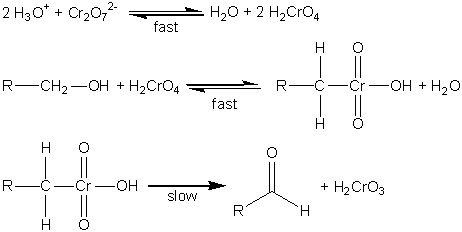
\includegraphics[width=1.0\linewidth]{gfx/4A}
		\end{center}
	\caption[Oxidation of Alcohol]{\label{4A_Equation}}
	\end{figure}


\section{Procedure}
	A 50\% ($v/v$) solution of $H_{2}SO_{4}$ was provided as `Solution A'. A 200 $\mu L/L$ solution of Ethanol was provided as `Solution B'. The following steps were then followed:
	\begin{enumerate}
		\item Weighed 20 $mg$ of $K_{2}Cr_{2}O_{7}$ and 25 $mg$ of $AgNO_{3}$ into a volumetric flask of 50 $mL$ using a funnel. Solution A was used to make the volume to 50 $mL$. The solution thus obtained was labelled `Solution C'.
		\marginpar{\Lisa Even if the mass is not very precise, it doesn't matter so long as the same volume of the solution is used, since the important factor here is change in concentration}
		\item Pipetted the following volumes in four separate 10 $mL$ volumetric flasks.
			\begin{enumerate}
				\item 7.5 $mL$ of solution C and 0.5 $mL$ of solution B
				\item 7.5 $mL$ of solution C and 1.0 $mL$ of solution B
				\item 7.5 $mL$ of solution C and 1.5 $mL$ of solution B
				\item 7.5 $mL$ of solution C and 2.0 $mL$ of solution B
			\end{enumerate}		
		And in another 10 $mL$ flask, pipetted 7.5 $mL$ of solution C and a volume unknown to other team members between 0.5 to 2.0 $mL$ of solution B.\\
		The volume was filled up using Solution A.
		\marginpar{\Lisa Take care to not accidentally include the extra `unmarked' volume while pipetting}
		\item Measured the absorbance as a function of alcohol concentration and estimated the concentration of unknown alcohol sample given.
	\end{enumerate}


\section{Observations}
Our experiment failed since the trend was unacceptable. We will repeat the experiment in the make-up lab, as was advised by our Professor.
\begin{flushright}
November 15, 2012
\end{flushright}
The experiment was repeated in accordance with the advice and the results are given in \autoref{E4A}. We had made a mistake in measurement and addition of solution B in the fourth solution; it hasn't thus been included in the result.

\begin{figure}[bth]
	\begin{center}
		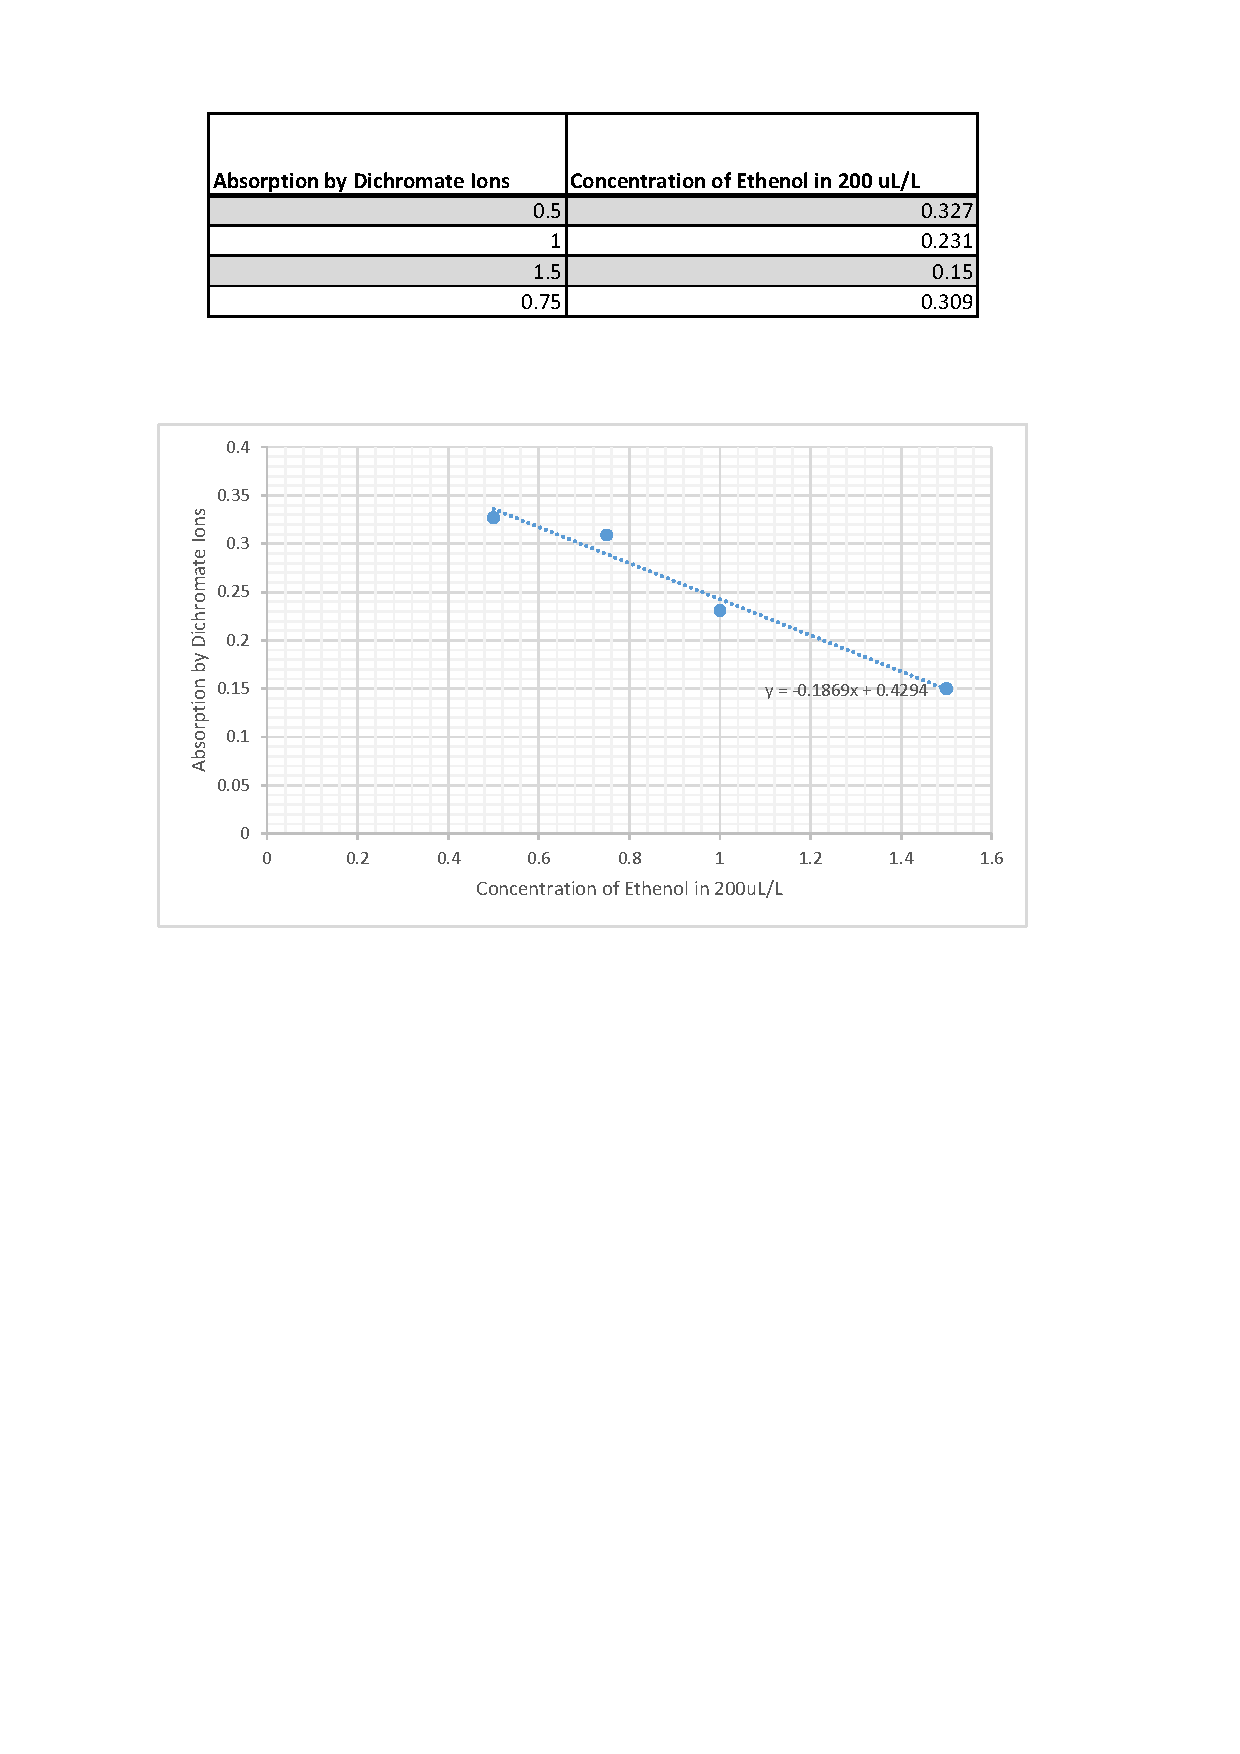
\includegraphics[width=1.15\linewidth]{gfx/makeup_lab}
	\end{center}
\caption[Dichromate's Absorption as a function of Alcohol Concentration]{\label{E4A}}
\end{figure}

\section{Acknowledgements}
I thank our PhD student guide, Ms. Shruti, who helped us with the performance of the UV-Vis Spectroscopy. I also acknowledge the contribution of my team members, Ms. Athira and Mr. Arpit, for performance of the experiment.

\begin{flushright}
November 15, 2012
\end{flushright}

I would like to thank Mr. Arpit for performing the experiment again with me. Also, I must acknowledge the contribution of our Lab Assistants who helped us operate the UV-Vis spectroscope. And as always, Prof. KSV is sincerely acknowledged.

\section{References}
\begin{enumerate}
	\item K. S. Visvanathan's Notes
\end{enumerate}